% !TeX spellcheck = en_US
those tips are collected from \href{https://www.carbon111.com/mwxt.html}{Carbon111}
\subsection{An Extra LFO from Modifiers}
A cool way to generate a third LFO to use for that extra touch of animation for your monster sound! Submitted by Rizacan.\\
An extra LFO won't disturb anyone! Here's a little LFO idea using Modifiers as below.
\bigskip % Add an empty line
%These are optional parameters to finetune the placement of tables and figures, with the following meaning:
%
%h, here
%t, top
%b, bottom
%p, page of float
%e.g. \begin{figure}[!htb]
\begin{figure}[ht!]
	\centering
	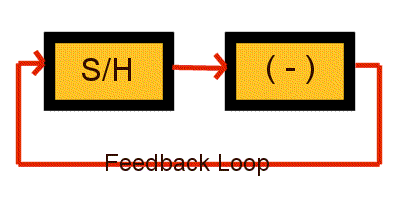
\includegraphics[width=90mm]{pics/lfo_feedback.png}
	\caption{Create a third LFO.}
	\label{third_lfo}
\end{figure}
S/H rate control input sets the overall frequency. Using the filter Modifier, you can get triangle waves. It can also be used for PWM, freeing up other LFOs for other uses!\\
Here are Two examples in Sysex format: \href{https://www.carbon111.com/sysex.zip}{two Examples}
The first one: ``ModifierLFO'' is a simple LFO example. Modifier 1 creates the squarewave and Modifier 3 smoothes the output of Modifier 1 (or 2).\\
The second one, ``Janmichelphaser'', is a simple solina string simulation with a phaser. Modifier 3 produces a triangle waveform using Modifier 1's square wave and modulates PW.
\subsection{Wavetable Browser}
A nice tutorial to create a patch that will allow you to fully audition each of the XT's wavetables. Actually rather handy! Submitted by vanHouten.\\
The following is a walk through for a simple patch that does nothing more than scanning a chosen wavetable as a whole by routing an LFO to the wave position.
\begin{enumerate}
	\item Search through the sounds to find one you don't ever want to hear again and initialize it by pressing ``play/shift'' and ``global'' simultaneously, then turn the main dial to the right until the display shows ``init sound ...'' $\to$ confirm with ``shift'' and ``global''.
	Now all parameters are set to their ``neutral'' positions. 
	\item Turn one of the oscillator's volume to zero and the other to a convenient level, so you can hear it!
	\item Choose wavetable \#51 ``1-2-3-4-5'' , go into the wavetable menu and set ``limit'' to ``on''. This way you can tell the oscillator not to trigger the last three waves of the wavetable, which are the basic synth wave forms at the end of every wavetable.
	\item Now in the mod-matrix: choose ``Mod1'' and set Wave1Pos for ``Destination'', ``Amount'' to +63 and ``Source'' to LFO1. This way the LFO modulates the number of the wave within the chosen wavetable being played.
	\item If reading this bores you by now: Then you have an idea how to finish this.
	\item Adjust LFO1 to a moderate speed like 52, ``Shape'' = sawtooth, ``Delay'' = Retrigger, ``Symmetry'' = +63.\\
	Background: Take a sawtooth wave as a waveform, which starts at a negative value, rises up linearly to the maximum positive amount and falls back to the starting point. By setting Symmetry to +63, the starting point is raised to zero and all following values are in the positive range $\to$ makes sense, as there are no negative wave-numbers in any wavetable. ``Retrigger'' makes the LFO initiate a new cycle, every time a note is played. Finished! If you hit a lower key and hear your machine say ``one two three four five'', everything works the way it should. (Wavetable \#52 says "nineteen twenty", but \#51 and \#52 are the only two speech wavetables of the microwave) Now you might save this patch as a kind of ``wavetable browser''.
	\item By playing a note (preferably a lower one), the LFO starts to run from 0 to it's maximum value and makes the oscillator play wave-\# 0-60 in a row, repeatedly. ``Limit'' prevents access of the basic waveforms at the end, so what you hear is just the full wavetable scan. By selecting another wavetable, you will hear the whole content of this wavetable. This way you can get familiar with the single wavetables and their properties. Of course you can also select the modwheel to be source for the start wave position in the Modulation Matrix and scan through the wavetables by turning it from minimum to maximum... With the settings already made in the Modulation Matrix, this will provide a complete scan as well. As every sound that comes out of you machine, comes first of all from the waves of the chosen wavetable. It is quite useful to have a rough idea of what each one sounds like, so you know which ones to use if you have an idea for a preset.
\end{enumerate}
\subsection{Formant Shift through Windowed Sync}
A great tip by Snyxol for a kind of "smoothed" hard sync that gives formant-type timbres.\\
You can do a smooth kind of formant shift on every waveform on the XT (and Virus, too, but not Q/mQ), and this without the need to create formant shift wavetables like “Chorus2” or “FormantVoc”. I refer to this method as “windowed sync”. It´s a combination of hard synchronisation and ring modulation. Although it is not really an accurate formant shift of the spectrum (this would require a very CPU/DSP intensive spectrum analysis through FFT, computing of the transformed spectrum and resynthesis by IFFT), it can sound rather similar. Dynamic, fat and nice evolving textures can be done by modulating “windowed sync” by a LFO or envelope.\\
Pure hard sync sounds pleasant on buzzy waveforms like saw and pulse, because these waves already have vertical transients. On smoother waveforms, however, it is poison for the ears, when sweeping the pitch of the sync slave (osc 2). It crackles like a scratched vinyl disc. This is because the harsh vertical transitions at the sync time points get smaller and bigger (depending on the phase) at wich the slave wave cycle breaks off to start a new cycle. Damping with a lowpass filter is not a good solution to reduce the harsh crackling. It would still be audible, though rounded, and the upper harmonics of the soft wave would be dampened.\\
Windowed sync: Eliminates the vertical transitions at sync time points more efficiently. The trick in steps:
\begin{itemize}
	\item Activate Sync
	\item Choose for Wave1 triangle or another soft waveform.
	\item In the mixer open only the RM signal.
\end{itemize}
\bigskip % Add an empty line
%These are optional parameters to finetune the placement of tables and figures, with the following meaning:
%
%h, here
%t, top
%b, bottom
%p, page of float
%e.g. \begin{figure}[!htb]
\begin{figure}[ht!]
	\centering
	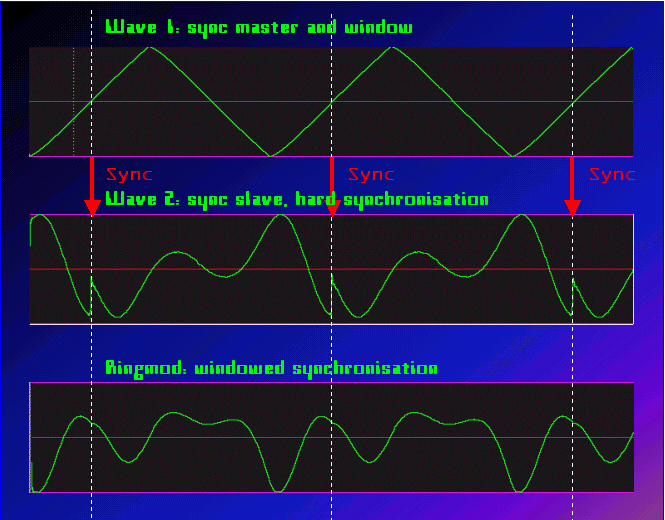
\includegraphics[width=90mm]{pics/format_shift_window_sync.png}
	\caption{Removing the vertical transitions at sync time points more efficiently}
	\label{Formatshift_window_sync}
\end{figure}
Ringmodulation (RM) is synonymous \notes{Thats not true, RM is something completely different than AM?!} with amplitude modulation. It multiplies both input signals samplewise. Thus you can consider Wave1 as an amplitude envelope of Wave2. Exactly when the sync master (Osc1) starts a new cycle and forces the slave osc (Osc2) to start a new cycle, too, the triangle wave crosses the zero axis. Thus the RM signal has amplitude 0 at the sync time points, and the discontinuities in the Wave2 signal are faded out. The result is a soft, continuous wave, mostly round, sometimes with a little edge like on a triangle wave, but not harsh. In other words, Wave1 has the task of a window function, a window that let´s through the “clean” parts of the wave while hiding the dirty sync jumps.\\
The good thing is that the triangle wave is present in all wavetables. Of course you can use another wave as window, if there is a suitable one in the wavetable. Suitable are smooth waves without steep transients, i.e. sine and dull organ waves.\\
The level of the RM signal is often rather low, because the amplitudes of the triangle wave and often that one of Wave2 are not normalized. The volume can be amplified with the $\sin(x)$-LP filter or the Waveshaper filter with square as shaper wave and a very small RM level (ca. 4-10).
\subsection{How program Airy Sounds}
Here's some excellent guidelines to help you create "airy", breathy sounds on the XT. Submitted by Nifflas.\\
I've experimented a lot with "airy" sounds the last days. I think most of you already know of this way of doing it, but in case you've never tried this:
Turn on only the noise generator. Lower the cutoff a bit, and set keytrack to 100\%. Set filter resonance to a very high value, but not so high that it self-oscillates. You will need to tweak the second filter a little bit since you're working with noise.
And of course play around with the ADSR envelope and add some effects, etc.
If you've done it right you have a very "airy" sound now. Here are some more things you can do with it.
Use the LP/BP filter and set the BP offset to +7 (Sounds great for pads) Or why not try the sinus or waveshaper?
\paragraph{Airy sounds part I:}
It's not easy to make the wave generators itself to sound airy, but there is one way to do it, without even using any oscillators.

Start with ``Init Sound (V1.1)''
\begin{itemize}
	\item Set Wave1 mix and Wave2 mix to 0
	\item Set Noise mix to 24
	\item Select the 24dB BP filter
	\item Set Cutoff to 71 and Resonance to 112
	\item Set Cutoff keytrack to +100\%
\end{itemize}
This is a very nice starting point for making airy sounds.
Two Hints:
\begin{enumerate}
	\item The Dual L/BP filter, with BP offset +7 sounds really cool.
	\item Always experiment with the second filter, it can often improve the sound a lot. 
\end{enumerate}
\paragraph{Airy sounds part II:}
One way to make airy sounds with many synthesizers is to let a noise generator frequency modulate an oscillator. However, this can not be done by using the Microwave's noise generator, so let's turn Wave Generator 2 into a noise source instead. Start with ``Init Sound (V1.1)'':
\begin{itemize}
	\item Set Wave1 mix to 0 for now.
	\item Choose a wavetable which is harmonic rich and chaotic. Wavetable \#46 ``Heavy Fuzz'' is just perfect.
	\item Tune Oscillator 2 to -3 octaves.
	\item Set Oscillator 2 keytrack to 0\%
	\item Set Wave2 startwave to 31
	\item Set LFO1 shape to random, and speed to 127.
	\item Mod matrix slot 1 - Source: LFO1 Amount: +55 Destination: Wave2 Pos
\end{itemize}
This is chaotic, random waves are being picked like mad from the wavetable. However, this is not chaotic enough.\\
Mod Matrix slot 2 - Source: LFO1 Amount: +40 Destination: Osc2 Pitch\\
Now it is.
\begin{itemize}
	\item Set Wave2 mix to 0
	\item Set Wave1 mix to 70
	\item Set Wave1 startwave to Triangle
	\item Set FM amount to 20
\end{itemize}
Enjoy the result. Use this as a starting point for making airy sounds.\\
A few hints:
\begin{enumerate}
	\item Try other waves, like sawtooth, square, or waveforms from the wavetable.
	\item Try other wavetables for other noise characteristics.
	\item When using some wavetables you might not want LFO1 to control both Wave2 pos and Oscillator 2 Pitch. To not consume another LFO, use Modifier Delay to delay LFO1 a little bit, and use the delayed source to control Wave2 pos.
\end{enumerate}
\subsection{Frequency Ratios for Waldorf synthesizers (Microwave II,xt(k), micro Q, Q)}
More of Alexander Eslava's handiwork. These frequency tables provide specific settings needed for Ring Mod, FM and other types of effects. These very usefull tables have been translated by Bodo Koktanek. \notes{I have added some definitions for variables in the formulas and typed formulas more mathematically, this should help with overview. I wont use real fractions these can get very small, when printing it out.}
\subsubsection{Frequency Ratios}
ALL FREQUENCY RATIOS UP TO the ratio $31/32$, which is 5 Octaves.\\
frequency ratios between 2 oscs consisting of natural numbers are important to make harmonic chords/layers, FM, RM and filter-FM.
to the ear, a harmonic spectrum is not necessarily percepted as consonant. to sounds consonant, the numerator or the denomiator of the frequency fraction $f_1/f_2$ must be a very small number (1 to 5 (?)). \notes{What is meant with $f_1$ and $f_2$?}\\
Pitch difference in semitones ("delta pitch"): $DP = 12 \cdot \ln(f_2/f_2)/\ln(2)$, this means: osc2 is pitched DP semitones higher than osc1.
The table maps every freq-ratio between Osc1 and Osc2 to the pitch offset of $f_2$ relative to $f_1$.
\begin{example}[using the table (microwave2)]
	To get a freq ratio of $f_1 / f_2 = 2 / 13$ look up in the table and set the pitch of osc2 by 3 octaves, -4 semitones and +52 detune units higher than osc1. (unshortened fractions are eliminated)
\end{example}
in the table always f1f2: swap f1 and f2, read the values in the table and then invert the sign of those values.
expl: f1:f2 = 7:4
--swap--> f1:f2 := 4:7
---read---> oct=1, sem=-2, det=-40
---invert sign---> result: oct=-1, sem=+2, det=+40
\todo{Lots of tables to add from HTML files}
\subsubsection{Frequency Ratios for FM}
Let us call $f_C$ the Frequency of the Carrier and $f_M$ the frequency of the Modulator.\\
To generate only odd harmonics by osc- and/or filter FM, you have to follow the following rules:
\begin{enumerate}
	\item  Can select the modulator waveform arbitrary. (also waves with even harmonics, like sawtooth)
	\item the carrier osc waveform must consist of odd harmonics only. (i.e. triangle, square, sine)
	\item the frequency ratio must be in the form:
	$f_C / f_M = (2m-1) / 2n \for m,n = 1, 2, 3, \dots$, which	means: $f_C / f_M = \odd / \even$ frequencies.
	\item the carrier-signal must be the only one turned up in the mixer of the osc-section.
\end{enumerate}
Note: These rules are reversed to those of odd harmonic ringmod!
\begin{example}[Microwave 2/XT(k) or Q]
	we make both an osc-FM: osc2 $\to$ FM $\to$ osc1 and a filter-FM: osc2 $\to$ filter cutoff freq.\\
	Set osc2 - 1 octave higher than osc1 octave value ($f_C / f_M = 1 / 2$), select triangle or square as wave1 and modulate FM amount or cutoff.
\end{example}
\begin{example}[for XT]
	Wavetable 5 (square sweep) is good as carrier and modulator:
	\begin{itemize}
		\item As carrier: you can gradually change from clean to buzzy.
		\item As modulator: the upper waves (near square) sound more squechy, brighter, whereas the lower waves (near sine) make the fm darker and somewhat noisier.
	\end{itemize}
\end{example}
the table maps every freq-ratio betwenn carrier and modulator to the pitch offset of modulator relative to carrier.
\begin{example}[using the table (microwave2)]
	To get a FM ratio of $f_C / f_M = 2 / 13$ look up in the table and set the pitch of the modulator by 3 octaves, -4 semitones and +52 detune units higher than the carrier.
\end{example}
\todo{Lots of tables to add from HTML files}
\subsubsection{Frequency Ratios for RM}
Here is a way through ringmodulation (RM) to transform arbitrary waves into new ones containing only odd harmonics (somewhat hollow, clean, aetherical sounding):\\
(since RM is the multiplication of 2 audio-signals, both oscillators can be threated the same way, unlike in FM, where one is the carrier, the other one the modulator. Despite of that in these notes, call the ringmodulating Oscs "Carrier" and "Modulator". they can be swapped. Take for the Microwave 2: osc1 as carrier, or osc2 if prefered.)
to generate odd harmonics, you have to follow the following rules:
\begin{enumerate}
	\item Can select the carrier waveform arbitrary. (also waves with even harmonics, like sawtooth)
	\item the modulator osc waveform must consist of odd harmonics only. (i.e. triangle, square, sine)
	\item the frequency ratio must be in the form: \notes{What is $f_C$?}
	$f_C / f_M = 2m / 2n-1 \for m,n = 1, 2, 3,\dots$
	means: $f_C / f_M = \even / \odd$
	\item the RM-signal must be the only one turned up in the mixer of the osc-section.
\end{enumerate}
And a short example:
\begin{example}[Microwave 2/XT(k)]
	Set Osc2 1 octave deeper than Osc1, select Triangle as Wave2, wavetable \#64 ``chorus2'' and make a wavetable-sweep on wave \#1.
\end{example}
The wavetable maps every freq-ratio between carrier and modulator to the pitch offset of modulator relative to carrier.
\begin{example}[example for using the table (microwave2 )]
	To get a RM ratio of $f_C\colon f_M = 2 / 13$ look up in the table and set the pitch of the modulator by 3 octaves, -4 semitones and +52 detune units higher than the carrier.)
\end{example}
\todo{Lots of tables to add from HTML files}
\subsection{Applying Glide To One Oscillator Only}
A great way to achieve a very unique sounding glide effect! Submitted by Nifflas.
\begin{itemize}
	\item Set Keytrack for both Oscs to 0\%
	\item Activate Glide
	\item Mod Matrix: Keyfollow $\to$ Osc1 pitch (+56) and Keytrack $\to$ Osc2 pitch (+56)
\end{itemize}
This can be very useful. Only osc1 will be affected by the glide.
\subsection{Sample \& Hold}
Some nice guidelines for using S \& H on the XT. Submitted by Snyxol.\\
To obtain the same timbre on every note's pitch, Keyfollow must modulate S \& H Rate with Amount +56.\\
It is even possible to make the S\& H sound harmonic (periodic waveform): Set S \& H Rate to 91 (or add -24, -12, +12, 24, etc.. Every 12 units the S \& H rate doubles) and Osc Pitch to octave = semitone = detune = 0.\\
Important! Quantize (in the quality menu) must be 0. (Otherwise, the pitches of the Oscs would deviate because of the quantization mechanism.)
\begin{example}
	killer robot voice with above settings and wavetable ``Chorus2''; modulate the wavetable with an envelope!
\end{example}
\subsection{Unisono Speed Modulation}
A cool tip with example regarding the modulation of the Unisono "spread" parameter - how fat do you want it!? Submitted by Snyxol.\\
Here is a trick to modulate Unisono spread by LFO, Envelope, Modwheel, etc.:

Don't use the normal spread. Instead, use an unsynced random-LFO as a spread source. These random values are different in each voice and are mostly evenly distributed.
\begin{example}
	fat saw lead, the "fatness" is slowly modulated by LFO 1, while LFO 2 serves as the spread source:
	\begin{itemize}
		\item poly, unisono, spread = 0
		\item LFO 1: Sync: on/Clock (!!!) (phases must be equal in all voices), Rate: 20, shape: Sin/Tri
		\item LFO 2: Sync: off (!!!) (phases must be different in all voices), Rate: 0 (but at first you must set it for a short time to a higher value), Shape: Random
		\item In Mod Matrix Mod 2: Src: LFO 1 (or Envelope, Modwheel, etc.), Amnt: +46, Dest: M3 Amnt
		\item Mod 3: Src: LFO 2, Amnt: 0 (or other value for asymmetry), Dest: Pitch
	\end{itemize}
\end{example}
\subsection{Pitch Independent Phasing}
Here's an interesting couple of methods for the control of oscillator phasing (beating) independent of pitch. Submitted by Snyxol.\\
(Its assumed the phase drifting effect caused by detune is called "phasing".)
If 2 oscillators have constant (not modulated) detune, the phasing rate is bigger at higher pitch, more precisely: phasing rate relates exponentially to pitch and doubles at each octave.
For certain sounds, a constant pitch-independent phasing rate would be desirable.
Here is one solution that achieves it:
\begin{itemize}
	\item (drawback: it needs the Modwheel or one of the CCs W,X,Y,Z to set detune)
	\item Oscillators: same wave, exactly (!) same pitch, no detune
	\item Mixer: both waves at same level (63)
	\item Mod Matrix:
	\begin{itemize}
		\item Mod 3: Src: Modwheel; Amnt: +17; Dest: Osc2 Pitch
		\item Mod 4: Src: Keyfollow; Amnt: -45; Dest: M3 Amount
	\end{itemize}
\end{itemize}
The modwheel sets the phasing rate.\\
Here's another implementation that does not require the Modwheel:
\begin{itemize}
	\item Oscillators: same wave, exactly (!) same pitch, no detune
	\item Mixer: both waves at same level (63)
	\item Mod Matrix:
	\begin{itemize}
		\item Mod 3: Src: maximum; Amnt: -17 (or whatever); Dest: Osc1 Pitch
		\item Mod 4: Src: maximum; Amnt: +17 (or whatever); Dest: Osc2 Pitch
		\item Mod 5: Src: Keyfollow; Amnt: +45; Dest: M3 Amount
		\item Mod 6: Src: Keyfollow; Amnt: -45; Dest: M4 Amount
	\end{itemize}
	\item This uses more Modulation slots.
\end{itemize}
You set the phasing rate by the amounts of M3/4, both must have the same absolute value and M3 must be negative and M4 positive.
\subsection{Comb+ Filter Simulation}
An ingenious way to simulate a positive comb filter. For those of you envious of the Q/micro Q's comb filter, this is a pleasant surprise! Submitted by Snyxol.\\
On the MW2/XT can emulate a comb+ filter without resonance (mono chorus) modulated by Envelope/LFO/whatever:
The mod source (in this example: Free Envelope) shifts the relative phase between both Oscs. It behaves the same as a 1-Osc-synth with Comb+ Filter.
If the stages of the Envelope have different slopes, the fatness changes between them. When you apply the normal chorus in addition, you can get mindblowing fat phasing. Sounds cool with Saw, Sqr and Chorus2.
The case of Sqr is particularly interesting: The sum of 2 phase shifting square waves is a symmetric PWM pulse wave, containing only odd harmonics; the free envelope controls the pulse width.
\begin{itemize}
	\item Oscillators: same wave, exactly (!) same pitch, no detune
	\item Phase 1: 3°
	\item Phase 2: try out!
	\item Mixer: both waves at same level (63)
	\item Trigger2 mode: Poly; assign: Normal
	\item Mod Matrix:
	\begin{itemize}
		\item Modifier 2: Src 1: modify \#4; Type: Filter; Param: 120
		\item Modifier 3: Src 1: modify \#2; Src 2: Modwheel; Type: *
		\item Modifier 4: Src 1: Free Env; Type: diff
		\item Mod 1: Src: modify \#3; Amnt: -36; Dest: Osc1 Pitch
		\item Mod 2: Src: modify \#3; Amnt: +36; Dest: Osc2 Pitch
		\item Mod 3: Src: Keyfollow; Amnt: -45; Dest: M2 Amount
		\item Mod 4: Src: Keyfollow; Amnt: +45; Dest: M1 Amount
	\end{itemize}
\end{itemize}
Set the mod depth of phase with Modwheel, and set starting point of phase modulation with the phases of both Oscs. Here's how it works:
\begin{itemize}
	\item Mod 1..4: see ``Pitch Independent Phasing'' and ``Frequency as Mod Source''.
	\item To move the relative phase the Oscs must be detuned.
	The phasing speed is proportional to the frequency difference (not detune!) of the Oscs.
	\item Mod 3/4 make the frequency difference pitch independent.
	\item Modifier 4: the slope of the free envelope must be proportional to the phasing speed $\to$ the Envelope must first be differentiated and then it must modulate the frequency difference.
	\item Modifier 2: before the differentiated envelope modulates the frequency difference, it is smoothed to reduce abrupt fatness changes between the stages.
\end{itemize}
\subsection{FM Amount Guideline}
Some good information on the implementation of FM. Submitted by Snyxol.\\
FM is linear and FM Amount is pitch independent $\to$ at higher pitches the impact is weaker $\to$ timbre is pitch dependent. It's also possible to keep the timbre independent of pitch by making FM Amount be proportional to the carrier frequency - FM Amount = 0:
\begin{itemize}
	\item Mod 1: Src: maximum; Amnt: +59 (or whatever, must be >0); Dest: FM Amount
	\item Mod 5: Src: Keyfollow; Amnt: +45; Dest: M1 Amount
\end{itemize}
If you want to modulate FM amount, modulate the M1 Amount, or exchange in M1 maximum by something else: LFO, Envelopes, Modwheel, ...